\chapter{Introduction}
\label{intro}

The aim of this project was to create a fully-functional DLX microprocessor, entirely designed using the VHDL hardware design language. A team of three people contributed to the development of a custom architecture that would reflect what was taught during the ``Microelectronic Systems'' course, including all the essential features plus some additional ones that came from necessity and/or simple personal interest.

The whole block consists of a pipelined structure made by five contiguous stages, each contributing to a different functionality in order for a single instruction to take place during the same amount of clock cycles:
\begin{enumerate}
\item \textbf{IF} — Instruction Fetch
\item \textbf{ID} — Instruction Decode/Register Fetch
\item \textbf{EXE} — Execute/Effective Address
\item \textbf{MEM} — Memory Access/Branch Completion
\item \textbf{WB} — Write Back.
\end{enumerate}

Each piece of information is represented by a 32-bits long \texttt{std\_logic\_vector}, which is also the required format for firmware commands. There's a total of 32 general-purpose registers, and the Datapath has been extended in order to include all the functionalities indicated in the advanced instruction subset. The Arithmetic Logic Unit was adapted as to be capable of performing all the related operations in a behavioral way as well.

All the rest of the Instruction Set is still compatible with the current implementation (even Floating Point operations), but all the ``unknown'' instructions will just resolve to a \emph{nop}: this way, it would become much easier to add the support for those ones as well if the project was to be resumed at a later time. As a matter of fact, after creating the required blocks, it becomes almost a matter of plug-and-play.

\begin{figure}[!ht]
\centering
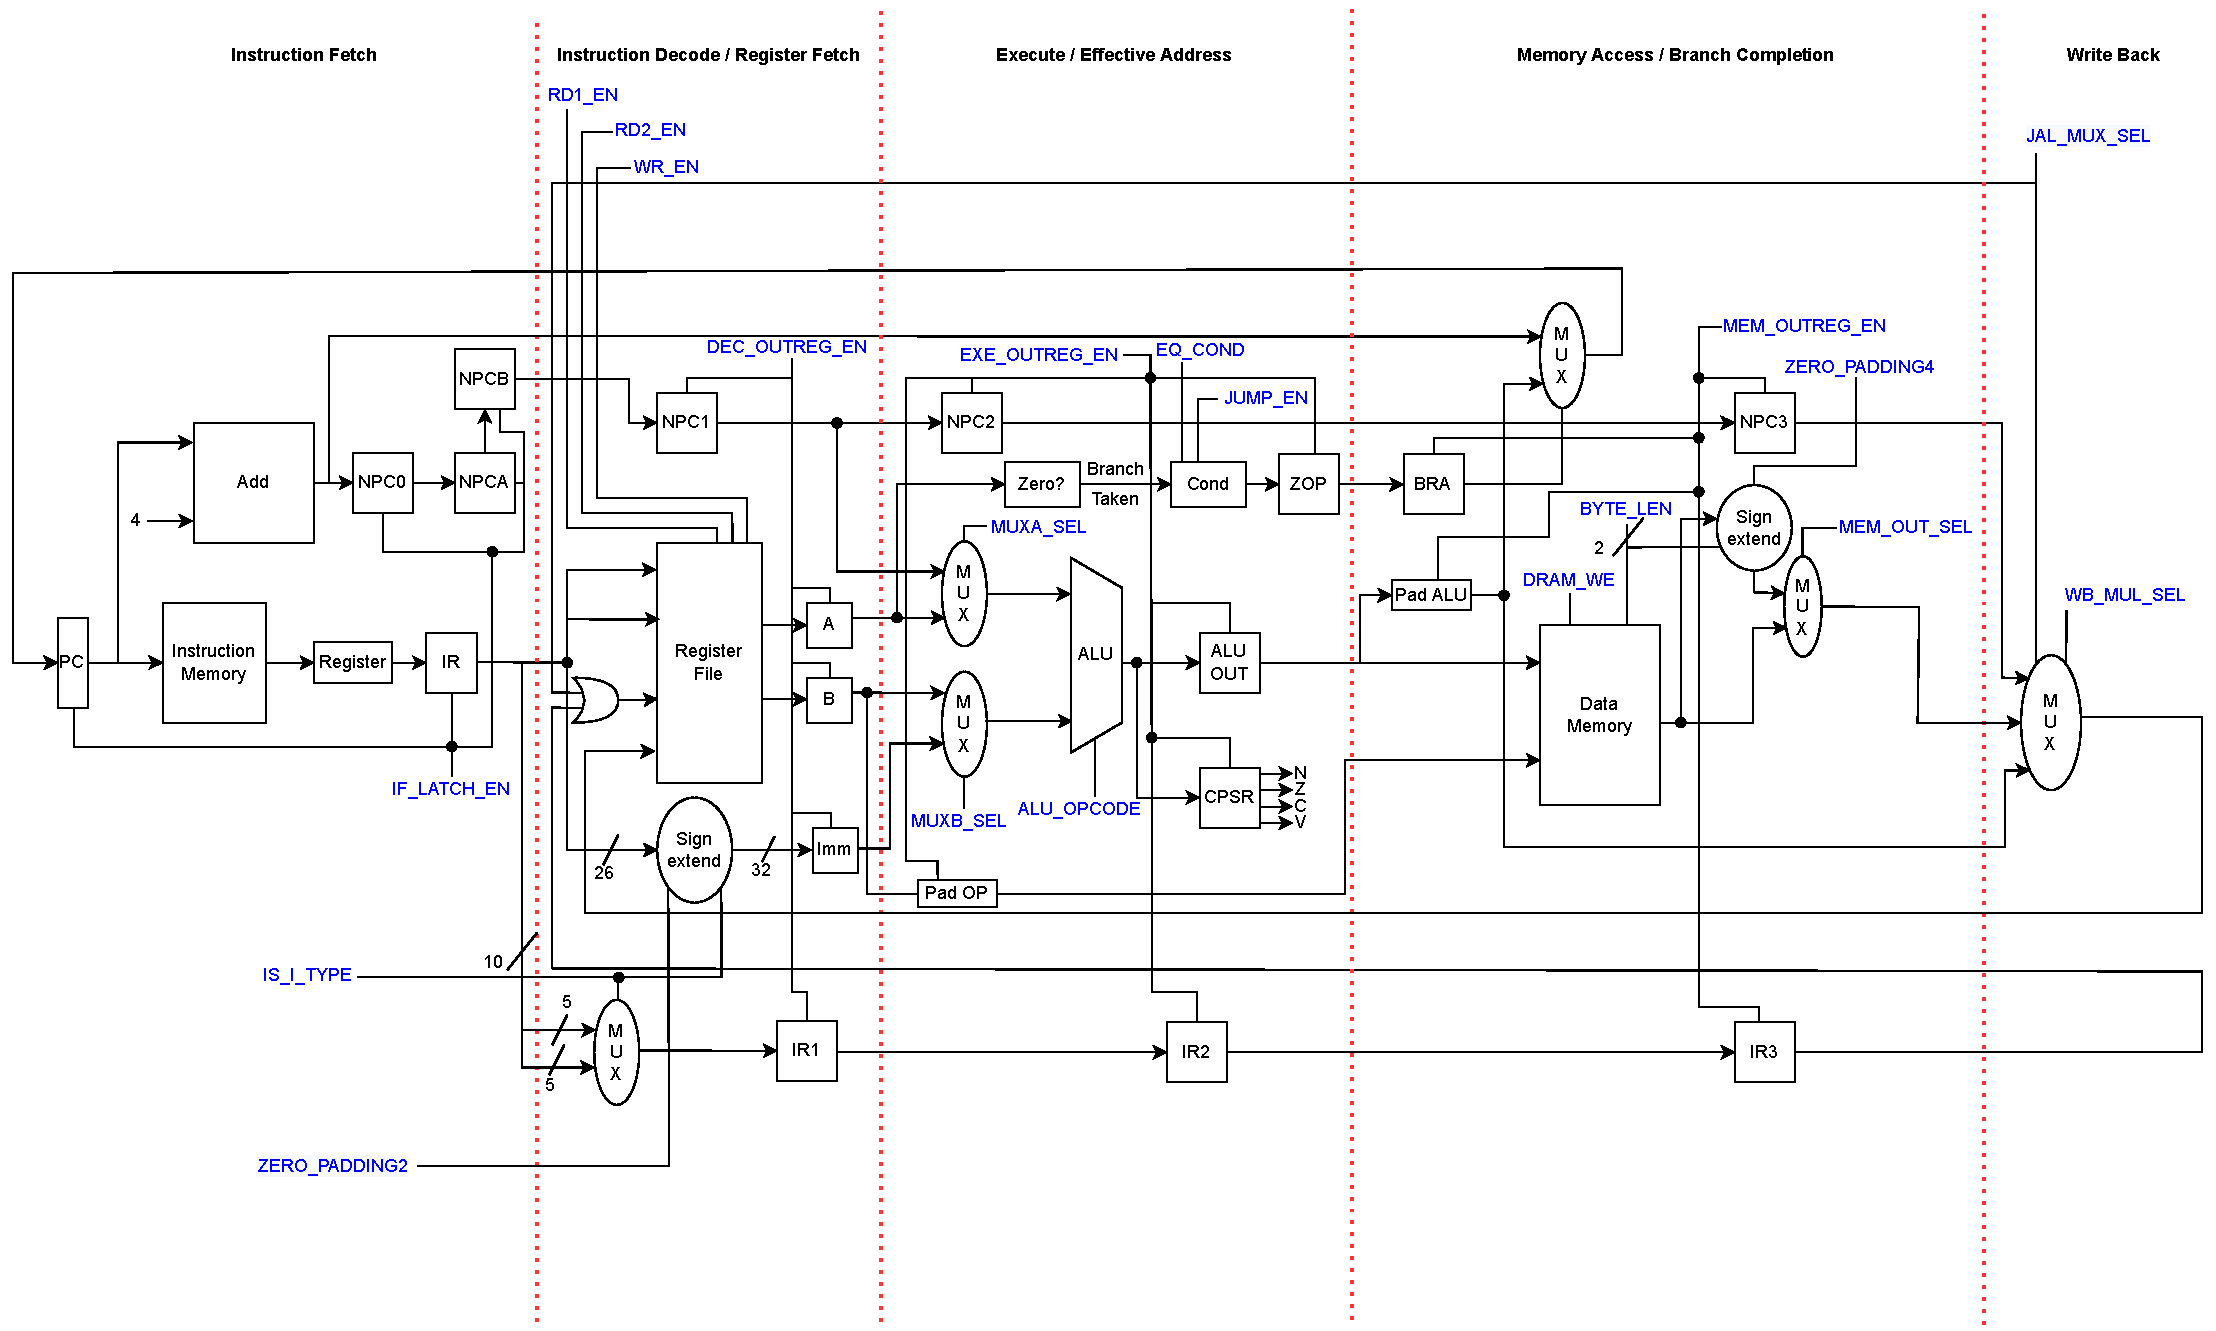
\includegraphics[width=\textwidth]{./chapters/figures/datapath.pdf} 
\caption{Overview of the main blueprint showing the current structure of the DLX.}
\end{figure}